\documentclass[a4paper,12pt]{report}
\usepackage{algorithmic}
\usepackage[linesnumbered,ruled,vlined]{algorithm2e}
\usepackage[margin=2cm]{geometry}
\usepackage[utf8]{inputenc}
\usepackage{listings} 
\usepackage{graphicx} 
\usepackage{color}
\usepackage{xcolor}
\usepackage{hyperref}
\usepackage{verbatim}
%\usepackage{mdframed}
\usepackage{multicol}
\usepackage{amsmath}
\usepackage[subnum]{cases}
\usepackage{stmaryrd}
\usepackage{nameref}

\setlength{\columnsep}{1cm}

\definecolor{codegreen}{rgb}{0,0.6,0}
\definecolor{codegray}{rgb}{0.5,0.5,0.5}
\definecolor{codepurple}{rgb}{0.58,0,0.82}
\definecolor{backcolour}{rgb}{0.95,0.95,0.92}

\lstdefinestyle{mystyle}{
    backgroundcolor=\color{backcolour},   
    commentstyle=\color{codegreen},
    keywordstyle=\color{magenta},
    numberstyle=\tiny\color{codegray},
    stringstyle=\color{codepurple},
    basicstyle=\ttfamily\footnotesize,
    breakatwhitespace=false,         
    breaklines=true,                 
    captionpos=t,                    
    keepspaces=true,                 
    numbers=left,                    
    numbersep=5pt,                  
    showspaces=false,                
    showstringspaces=false,
    showtabs=false,                  
    tabsize=2,
%     title=search.py,
    frame=single,	 
}

\lstset{style=mystyle}

\newcommand{\namedlisting}[2][]{%
    \lstinputlisting[caption={\texttt{\detokenize{#2}}},#1]{#2}%
}

\newcommand*\lstinputpath[1]{\lstset{inputpath=#1}}

\newcommand{\currentdata}{14 February 2015}
\newtheorem{example}{Example}

\begin{document}
\vspace{-5cm}
\begin{center}
Department of Computer Science\\
Technical University of Cluj-Napoca\\

\includegraphics[width=10cm]{fig/footer}
\end{center}
\vspace{1cm}
%\maketitle
\begin{center}
\begin{Large}
 \textbf{Artificial Intelligence}\\
\end{Large}
\textit{Laboratory activity}\\
\vspace{3cm}
Name: Fodor, Zsófia and Katona, Áron\\
Group: 30433\\
Email: fodorzsofi@yahoo.com katonaaron01@gmail.com\\
\vspace{12cm}
Teaching Assistant: Adrian Groza\\
Adrian.Groza@cs.utcluj.ro\\
\vspace{1cm}

\includegraphics[width=10cm]{fig/footer}
\end{center}

\tableofcontents

\chapter{A1: Search}

\section{Introduction}



\chapter{Bidirectional Search} 

Bidirectional search simultaneously searches from the start state to the goal state (\textbf{forward searching}) and from the goal state to the start state  (\textbf{backward searching}) hoping that these two searches will meet. The time and space complexity was reduced from $O(b^d)$ to $O(2 * b^{d/2}) = O(b^{d/2}) << O(b^d)$, where $b$ is the branching factor and $d$ is the depth of the shallowest solution.

\section{Implementation}


The algorithm uses the \textbf{Breadth-First Search policy}, meaning that it takes the shallowest node first. It stops when the forward and backward search intersect. If no solutions is found, than it returns \textit{None}.

We used two sets one representing the explored nodes that are still in the queue and another one, that contains the visited nodes that were popped out of the queue.
Entering the while loop, we firstly analyze the forward search. Take the next node from the corresponding queue and if it is not yet visited we put it in the visited set. After we have iterated through the nodes of the backward search, if there is a meeting point then we return the current path and the path accumulated by the backward search in reverse order.

Next we analyze the backward search the same way as we did for the forward search, the only difference being that we replace each action with its opposite action, we reverse the list containing them and add it to the accumulated path.

The motivation behind using sets is that they are more efficient than lists in verifying whether they contain an arbitrary element.

Source code: Appendix \ref{sec:code_bs}.

\begin{figure}[ht]
    \centering
    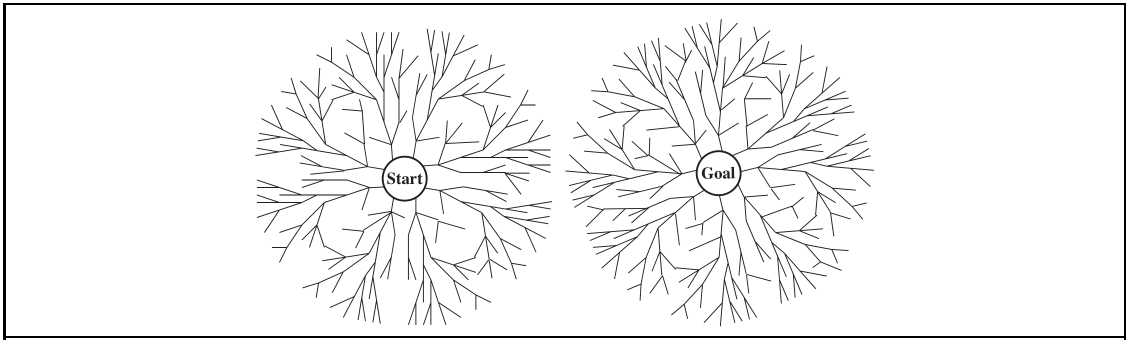
\includegraphics[width=.8\linewidth]{fig/bs.png}
    \caption{Visualization of the bidirectional search algorithm. \cite{aima2020}} 
    \label{fig:bs}
\end{figure}


\chapter{Iterative Deepening Depth-First Search} 

\section{Depth-Limited Search}
\label{sec:dls}

The depth-limited search is similar to the depth-first search, with the only difference, that a \textbf{depth bound} is added. Thus the algorithm searches for the goal state until the search tree's depth reaches the bound. If the bound is reached, the search backtracks to the parent node and continues searching in the next successor of the parent node. Therefore if there is a path to the goal, whose length is smaller than or equal to the bound, it will be found.

\subsection{Implementation}

To represent the nodes we used the \verb|Node| class, which is a simple data class whose \verb|state|,\verb|action| and \verb|cost| fields are used. More information about the class can be found in Appendix \ref{sec:nodes}.

The algorithm is a modified version of the recursive \textbf{depth-first search}. At each level of recursion, the function calls itself for all of the successors. The function returns not only the found goal node on success and None on error, but also an additional boolean parameter which specifies whether the search terminated because of a cutoff, or not. In each level of recursion, the limit is decremented. When it reaches 0, the returned cutoff value is true.

Source code: Appendix \ref{sec:code_dls}.


\section{Iterative Deepening Search}

The iterative deepening search strategies apply a search algorithm multiple times, with increasing bounds until the goal is reached. The calculation of the bound depends on the applied algorithm. We used the strategy of iterative deepening for the following search algorithms: depth-first search (\ref{sec:iddfs}) and A* (\ref{sec:idastar}).


\section{Iterative Deepening Depth-First Search}
\label{sec:iddfs}

Starting from an initial bound of 0, we call the depth-limited search and verify the returned result. In case a cutoff occurred, we increase the bound by one, and start again the search. If the goal node was found, the path from the start node which ends in the goal node is reconstructed and returned.

The algorithm is complete, because depth-first search, and in particular depth-limited search is guaranteed to find a solution, if the distance to the goal node is inside the bound. The bound is incremented from 0 indefinitely, thus if the solution exists, it will be found. 

The algorithm is optimal for unit action costs, because if no solution was found for bound $b$, the length of the shortest path from the start node to the goal node is at least $b+1$, and if there is any solution with length $b+1$, all of them are optimal solutions, and one of them will be found by the depth-limited search.

Source code: Appendix \ref{sec:code_iddfs}.



\section{Iterative Deepening A* Search}
\label{sec:idastar}

Iterative deepening is a preferred algorithm when we have a larger search state space than the one that can fit in memory and the depth of our solution is not known. 

Iterative Deepening A* is similar to A* the difference being that we do not keep all reached states in memory, at a cost of visiting some states multiple times. It is a very frequently used algorithm for problems that do not fit in memory, as stated above.

\subsection{Implementation}

The idea behind the algorithm was that we search the node with the lowest combined cost and heuristic first ($f = g + h$). The algorithm is limiting the size of the frontier by using this calculated f value as a bound.

We used a set in which we stored the visited nodes. Searching in sets is faster than searching in lists, that is why we chose set.
Besides this set, we used a list called path, that stored for each node its state, the action that needs to be performed to get there from the previous node and the cost.

We have a utility function that we call repeatedly until the returned value is either a very large number ($\infty$)  or  the \textit{None} state and we change the value of the bound to the returned value if none of these conditions is satisfied. 

The utility function begins with taking the last element from the path, computing the f value of this element and comparing it to the bound. If it is larger than the bound, we return the f value. If the state of the node is the goal state, it means we reached our goal, so we return the \textit{None} state. If none of these conditions are fulfilled, then we iterate through each child of the current node, add it to the visited set and to the path list, then we call the utility function on it. We make the adjustments according to the returned value of this call, remove the node from the visited list and the path. 
Lastly we return the minimum value which represents the minimum cost of all values that exceeded the current bound. 

\subsection{Remarks}

This algorithm was actually easy to implement after we understood the idea behind it. 

Comparing the number of expanded nodes we can see that it is much larger than for the A* algorithm, because of the fact that we do not keep all reached states in memory risking the fact that we might visit some nodes more than once. 

\chapter{Recursive Best-First Search} 

The recursive best-first search, similarly to the depth-limited search (\ref{sec:dls}), searches for the deepest node first, but stops after surpassing a bound. But in this case the bound is placed on the f-value of a node, instead of its depth.

The f-value of a node is the maximum between the f-value of its parent and the cost of reaching the node + the heuristic, i.e. $f(n) = max\{ g(n) + h(n), f(n.parent) \}$. When a branch of the search is cut off because the limit on the f-value, while backtracking, the f-value of a parent node will be updated with the f-value of its child. This way, the f-value of a node will become a more and more accurate estimation of the true cost of reaching the goal node from it.

This algorithm uses the principle of best-first searching. It only expands the node with the smallest f-value. If the node is on the current searching branch, than it will be expanded, otherwise the search tree backtracks to the level of the node with the smallest f-value. Therefore at each level of recursion we take the first two successors with the lowest f-value, call the search for the best option, and supply the bound as the f-limit of the alternative successor. This is repeated until the solution is found, or until the f-value of the best node will become greater than the f-limit. Thus it always considers a best and an alternative path, and switches between them, if the alternative path becomes the best one, in terms of lowest f-value.

The advantage of this algorithm is that it uses linear space: used for storing the nodes along the search path, and also the sibling of each node. The disadvantage is that it regenerates already visited nodes, which could happen very frequently. Thus it trades speed for storage.

For the implementation the \verb|Node| class (\ref{sec:nodes}) was used for storing the nodes, and a priority queue was used for obtaining the best successor of a node. The recursive function returns the result and None, if the goal node was found. If the goal was not found, it returns None and the f-value of the deepest node reached before surpassing the limit.

Source code: Appendix \ref{sec:code_rbfs}.

\begin{figure}[ht]
    \centering
    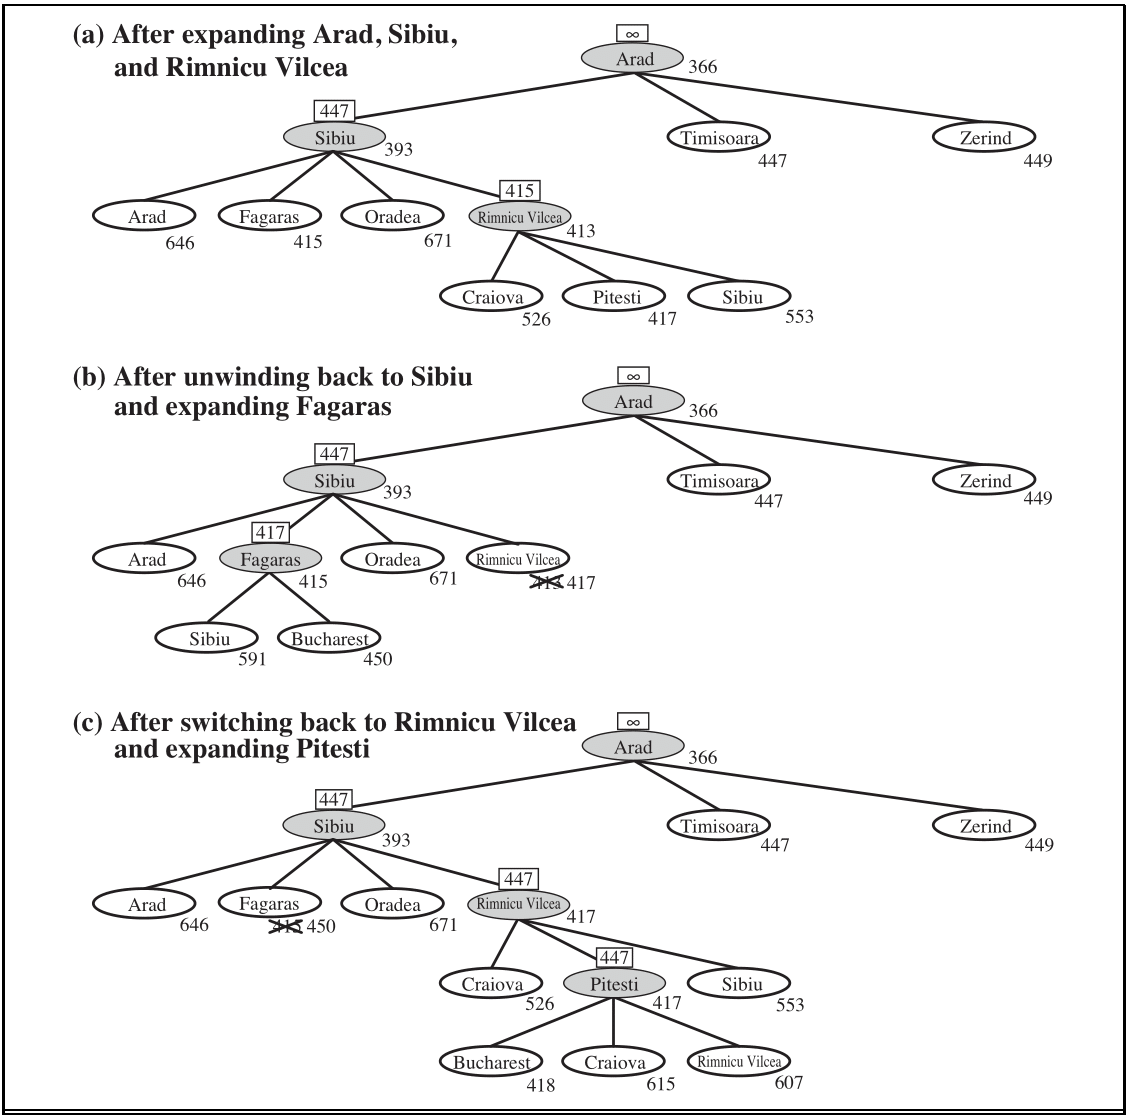
\includegraphics[width=\linewidth]{fig/rbfs.png}
    \caption{Finding a path from Arad to Bucharest by using recursive best-first search. The number above a node is its f-limit, and the number on the right of it is its f-value. The searching branch was switched two times. \cite{aima2020}} 
    \label{fig:rbfs}
\end{figure}


\section{Comparison} 

Consider $b$ the branching factor and $d$ the depth of the shallowest solution.


\subsection{Bidirectional Search vs Breadth-First Search}

As stated in chapter \ref{ch:bs}, the bidirectional search reduces the size of the frontier and the running time from $O(b^d)$ to $O(b^{d/2})$. To find a solution with length $d$, the two frontiers contain in the worst case only the nodes with the depth $d/2$ from either nodes. Thus both the space and the running time is reduced. 

However the implementation of the bidirectional search is difficult if the actions cannot be reversed fast. E.g. North $\leftrightarrow$ South.


\subsection{Iterative Deepening Depth-First Search}

\paragraph{vs Depth-First Search:}

The depth-first search does not find always the optimal solution, and may not find any solution even if it exists in the graph. However the iterative deepening version is optimal and complete, because each path is considered in increasing order of depth.

\paragraph{vs Breadth-First Search:}

The running time has the same $O(b^d)$ complexity. For the iterative deepening depth-first search the space complexity is reduced from $O(b^d)$ to $O(bd)$, because the deepest node is taken first. However because of the iterative deepening, the number of expanded nodes is higher.


\subsection{Iterative Deepening A* vs A*}

Iterative Deepening A* is similar to A* the difference being that we do not keep all reached states in memory, at a cost of visiting some states multiple times. It is a very frequently used algorithm for problems that do not fit in memory.


\subsection{Recursive Best-First Search}

\paragraph{vs A*:} 

RBFS uses only linear space, but suffers from frequently regenerating the nodes. Given enough time it could solve those problems that could not be solved by A* because of running out of memory.

\paragraph{vs Iterative Deepening A*}

The two algorithms are solutions for the same problem of reducing the size of the frontier of A*. Both suffer from revisiting  and regenerating nodes. However the RBFS is slightly more efficient, because of storing more information that the other one, thus increasing the speed.
 
 

\chapter{A2: Logics}

\section{Introduction}



\section{Logic via algebra} 

The article \cite{Ciraulo2020algebra} presents the theory about using algebra for solving logic puzzles. Below are summarized the parts that are used in this chapter.

0 and 1 represent the truth values ``false'' and respectively ``true''. $\llbracket P \rrbracket$ represents the truth value of the proposition $P$.

\begin{itemize}

\item $\llbracket P \rrbracket = 1 \iff P$ is true

\item $\llbracket P \rrbracket = 0 \iff P$ is false

\end{itemize}

The set $\{0, 1\}$ is:

\begin{itemize}

\item the smallest possible Boolean algebra

\item a distributive bounded lattice in which
every element has a complement

\item a Boolean ring: $x^2 = x \; \forall x$

\item a field of characteristic 2: $x + x = 0 \; \forall x$

\end{itemize}

Therefore any Boolean connective can be expressed as a polynomial. Table \ref{table:boolean_connectives} presents the connectives both in lattice and ring form. This table is used for translating the statements of the logic puzzles into equations. It is also used for the program which converts a Mace4 input file from propositional logic to modular arithmetic.

\begin{table}[h!]
\centering
\begin{tabular}{ rcl } 
 \hline
 CONNECTIVE & LATTICE form & RING form \\ 
 \hline
 Conjunction (AND) & $p \land q$ & $pq$ \\ 
 Exclusive disjunction (XOR) & $(p \lor q) \land \neg(p \land q)$ & $p + q$ \\  
 Inclusive disjunction (OR) & $p \lor q$ & $pq + p + q$ \\ 
 Negation & $\neg p$ & $p + 1$ \\ 
 Implication ($\rightarrow$) & $q \lor \neg p $ & $pq + p + 1$ \\  
 Biconditional ($\leftrightarrow$) & $(p \land q) \lor (\neg p \land \neg q)$ & $p + q + 1$ \\   
 Sheffer stroke (NAND) & $\neg (p \land q)$ & $pq + 1$ \\ 
 Pierce’s arrow (NOR) & $\neg (p \lor q)$ & $pq + p + q + 1$ \\ 
 \hline
\end{tabular}
\caption{Boolean connectives in the language of Boolean rings \cite{Ciraulo2020algebra}}
\label{table:boolean_connectives}
\end{table}

A logical puzzle is composed of statements in which an information about $A$ is equivalent with a predicate $P$. Can be written as:

\begin{center}
\begin{math}
a = p
\end{math}
\end{center}

Where $p = \llbracket P \rrbracket$ and $a$ has the truth value of that information about A, e.g. $a = \llbracket ``A \textrm{ is a knight}" \rrbracket$ 

Thus the puzzle can be written as a system of equations:

\begin{center}
\begin{math}
\begin{cases}
 a_1 = p_1\\
 \dots\\
 a_n = p_n
\end{cases}
\end{math} 
\end{center}

And can be reduced to the equation:

\begin{equation}
\prod_{i=1}^{n} (p_i + a_i + 1) = 1
\label{eq:one_eq}
\end{equation}

\section{Solving lady and tigers with algebra} 
\label{sec:puzzles}

In this section ``The Lady or Tiger'' puzzles are solved using both propositional logic and modular arithmetics in order to compare the two methods.

\subsubsection{Mace4}
\label{sec:mace4_flaw}

For verifying the correctness of the formulas written to solve the puzzle, we used mace4. Mace4 can solve the puzzles for both types of notations.

For the modular arithmetic input files we specified the following commands at the beginning, in order to configure arithmetic operations on the Boolean ring:

\begin{lstlisting}[numbers=none]
set(arithmetic).
assign(domain_size, 2).
\end{lstlisting}

However, mace4 has a flaw when using it for expressions on the Boolean ring. There are some cases in which mace4 does not give any result. To solve this, one must wrap those expressions with ``mod 2''. An example can be seen below:

\begin{multicols}{2}

\begin{lstlisting}[numbers=none,title=Input file that can be solved by Mace4]
set(arithmetic).
assign(domain_size, 2).
assign(max_models, -1).

formulas(assumptions). 
    m1 + m2 = 1.
end_of_list.
\end{lstlisting}

\columnbreak

\begin{lstlisting}[numbers=none,title=Mace4 output]
interpretation( 2, [number = 1,seconds = 0], [
    function(m1, [0]),
    function(m2, [1])]).
interpretation( 2, [number = 2,seconds = 0], [
    function(m1, [1]),
    function(m2, [0])]).
\end{lstlisting}

\end{multicols}


\begin{multicols}{2}

\begin{lstlisting}[numbers=none,title=Input file that cannot be solved by Mace4]
set(arithmetic).
assign(domain_size, 2).
assign(max_models, -1).

formulas(assumptions). 
    m1 + m2 + 1 = 0.
end_of_list.
\end{lstlisting}

\columnbreak

\begin{lstlisting}[numbers=none,title=Mace4 output]
=== Mace4 starting on domain size 2. ===

------ process 62347 exit (exhausted) ------
\end{lstlisting}

\end{multicols}


\begin{multicols}{2}

\begin{lstlisting}[numbers=none,title=Input file made to be solvable by Mace4]
set(arithmetic).
assign(domain_size, 2).
assign(max_models, -1).

formulas(assumptions). 
    (m1 + m2 + 1) mod 2 = 0.
end_of_list.
\end{lstlisting}

\columnbreak

\begin{lstlisting}[numbers=none,title=Mace4 output]
=== Mace4 starting on domain size 2. ===

------ process 62531 exit (all_models) ------
interpretation( 2, [number = 1,seconds = 0], [
    function(m1, [0]),
    function(m2, [1])]).
interpretation( 2, [number = 2,seconds = 0], [
    function(m1, [1]),
    function(m2, [0])]).
\end{lstlisting}

\end{multicols}

For simplicity, we will omit the wrapping by ``mod 2'' in this chapter.

The source files in the Mace4 input format can be found in annex \ref{sec:code_puzzle}.






\subsubsection{Representation}


In \textbf{propositional logic} we can represent the state of the $i$-th room by the following predicates:

\begin{itemize}

\item $li$: There is a lady in room $i$.
\item $ti$: There is a tiger in room $i$.
\item $mi$: Message on the door of room $i$
 
\end{itemize}

Then one must specify, that if the room contains a lady, it does not contain a tiger, and viceversa.

\begin{lstlisting}[numbers=none]
l1 -> -t1.
l2 -> -t2.
\end{lstlisting}


For representing the rooms in \textbf{modular arithmetics} we can define:

\begin{itemize}

\item 
\begin{math}
ri = [[``\textrm{There is a lady in room } i"]] = 1 +  [[``\textrm{There is a tiger in room } i"]] 
\end{math}


\item 
\begin{math}
mi = [[``\textrm{Message on the door of room } i"]]
\end{math}
 
\end{itemize}

In this representation the appearance of a lady and a tiger in the same room is implicitly exclusive.

These representations will be used in the following puzzles, unless it is specified otherwise.









\subsection{The first trial}

\subsubsection{Knowledge base}

The following statements are given:

\begin{enumerate}

\item Each of the two rooms contained either a lady or a tiger, but it could be that there were tigers in both rooms, or ladies in both rooms.

\item \textbf{Message on door 1:} In this room there is a lady, and in the other room there is a tiger

\item \textbf{Message on door 2:} In one of these rooms there is a lady, and in one of these rooms there is a tiger

\item One of the messages is true, but the other one is false

\end{enumerate}

The first statement enumerates all four possibilities. It does not give more information than the one included in the representation.

The second statement represents the truth value of the first message. It can be written the following forms:

\begin{multicols}{2}

\begin{lstlisting}[numbers=none,title=Propositional logic]
m1 <-> l1 & t2.
\end{lstlisting}

\begin{lstlisting}[numbers=none,title=Modular arithmetics]
m1 = r1 * (r2 + 1).
\end{lstlisting}

\end{multicols}

One can observe that logical equivalence was replaced with equality, conjunction with multiplication, and negation with an addition by one.

The second message states that at least one tiger and at least one lady exists. Because there are only two rooms, this means that one room contains a lady, and the other one contains the tiger. Thus we can use the XOR operator between \verb|r1| and \verb|r2| to force exclusivity, which in the case of the modulo 2 algebra it is represented by the ''+`` symbol.

\begin{multicols}{2}

\begin{lstlisting}[numbers=none,title=Propositional logic]
m2 <-> (l1 | l2) & (t1 | t2).
\end{lstlisting}

\begin{lstlisting}[numbers=none,title=Modular arithmetics]
m2 = r1 + r2.
\end{lstlisting}

\end{multicols}

As for the fourth statement, we simply need to specify that the two messages are not equal, i.e. the first is equal with the negation of the second. Or we can say that the two does not take the same value simultaneously (XOR).

\begin{multicols}{2}

\begin{lstlisting}[numbers=none,title=Propositional logic]
m1 <-> -m2.
\end{lstlisting}

\begin{lstlisting}[numbers=none,title=Modular arithmetics]
m1 + m2 = 1.
\end{lstlisting}

\end{multicols}



\subsubsection{Resolution}

The advantage of the modular arithmetics is that it can be resolved by algebraic methods, taking into consideration the rules of the boolean ring.

The system of equations representing the knowledge base:

\begin{numcases}{}
 m1 = r1 * (r2 + 1) \label{eq:p1_m1}\\
 m2 = r1 + r2 \label{eq:p1_m2}\\
 m1 + m2 = 1 \label{eq:p1_m1m2}
\end{numcases}

By replacing $m1$ and $m2$ in \ref{eq:p1_m1m2} we obtain:

\begin{center}
\begin{math}
 r1 * (r2 + 1) + r1 + r2 = 1
\end{math} 
\end{center}

Which can be rewritten as 

\begin{center}
\begin{math}
 r2 * (r1 + 1) + r1 + r1 = 1
\end{math} 
\end{center}

Knowing that $x + x = 0$ and $x + 0 = x$, we can omit the $r1+r1$ term form the equation and obtain:

\begin{center}
\begin{math}
 r2 * (r1 + 1) = 1
\end{math} 
\end{center}

In order to satisfy the equation, both operands of the multiplication must be 1. Otherwise the product would be 0. Therefore the result will be:

\begin{center}
\begin{math}
\begin{cases}
 r1 = 0\\
 r2 = 1
\end{cases}
\end{math} 
\end{center}








\subsection{The Second Trial}

\subsubsection{Knowledge base}

\begin{enumerate}

\item Each of the two rooms contained either a lady or a tiger, but it could be that there were tigers in both rooms, or ladies in both rooms.

\item \textbf{Message on door 1:} At least one of these rooms contains a lady.

\item \textbf{Message on door 2:} A tiger is in the other room.

\item The messages are either both true or both false.

\end{enumerate}


The first message tells us, that either one of the rooms contains a lady, or both of the rooms contain a lady.


\begin{multicols}{2}

\begin{lstlisting}[numbers=none,title=Propositional logic]
m1 <-> (l1 | l2).
\end{lstlisting}

\begin{lstlisting}[numbers=none,title=Modular arithmetics]
m1 = r1 * r2 + r1 + r2.
\end{lstlisting}

\end{multicols}


One can observe that the logical OR operator is replaced by multiplying the two terms, then adding each one of them. 


The second message tells us, that in the other room (i.e.: the first room) there is a tiger.
Here the negation will be replaced with an addition by one.

\begin{multicols}{2}

\begin{lstlisting}[numbers=none,title=Propositional logic]
m2 <-> t2.
\end{lstlisting}

\begin{lstlisting}[numbers=none,title=Modular arithmetics]
m2 = r1 + 1.
\end{lstlisting}

\end{multicols}

For the last statement we simply have to specify that the truth value of the two messages is the same.

\begin{multicols}{2}

\begin{lstlisting}[numbers=none,title=Propositional logic]
m1 <-> m2.
\end{lstlisting}

\begin{lstlisting}[numbers=none,title=Modular arithmetics]
m1 = m2.
\end{lstlisting}

\end{multicols}


\subsubsection{Resolution}

The system of equations representing the knowledge base:

\begin{numcases}{}
 m1 = r1 * r2 + r1 + r2 \label{eq:p2_m1}\\
 m2 = r1 + 1 \label{eq:p2_m2}\\
 m1 = m2 \label{eq:p2_m1m2}
\end{numcases}

By replacing $m1$ and $m2$ in \ref{eq:p2_m1m2} we obtain:

\begin{center}
\begin{math}
 r1 * r2 + r1 + r2 = r1 + 1
\end{math} 
\end{center}

Which can be rewritten as: 

\begin{center}
\begin{math}
 r2 * (r1 + 1) = 1
\end{math} 
\end{center}


In order to satisfy the equation, both operands of the multiplication must be 1. Otherwise the product would be 0. Therefore the result will be:

\begin{center}
\begin{math}
\begin{cases}
 r1 = 0\\
 r2 = 1
\end{cases}
\end{math} 
\end{center}







\subsection{The Third Trial}

\subsubsection{Knowledge base}

\begin{enumerate}

\item Each of the two rooms contained either a lady or a tiger, but it could be that there were tigers in both rooms, or ladies in both rooms.

\item \textbf{Message on door 1:} Either a tiger is in this room or a lady is in the other room.

\item \textbf{Message on door 2:} A lady is in the other room.

\item The messages are either both true or both false.

\end{enumerate}


The first message tells us, that either a tiger is in the first room, or a lady is in the second room. By double negation and De Morgan's Law we obtain: "It's not true that a lady is in the first room and a tiger in the second".


\begin{multicols}{2}
\begin{lstlisting}[numbers=none,title=Propositional logic]
m1 <-> t1 | l2.
\end{lstlisting}

\begin{lstlisting}[numbers=none,title=Modular arithmetics]
m1 = r1 * (r2 + 1) + 1.
\end{lstlisting}

\end{multicols}

The second message tells us, that in the other room (i.e.: the first room) there is a lady.

\begin{multicols}{2}

\begin{lstlisting}[numbers=none,title=Propositional logic]
m2 <-> l1.
\end{lstlisting}

\begin{lstlisting}[numbers=none,title=Modular arithmetics]
m2 = r1.
\end{lstlisting}

\end{multicols}

For the last statement we simply have to specify that the truth value of the two messages is the same.

\begin{multicols}{2}

\begin{lstlisting}[numbers=none,title=Propositional logic]
m1 <-> m2.
\end{lstlisting}

\begin{lstlisting}[numbers=none,title=Modular arithmetics]
m1 = m2.
\end{lstlisting}

\end{multicols}


\subsubsection{Resolution}

The system of equations representing the knowledge base:

\begin{numcases}{}
 m1 = r1 * (r2 + 1) + 1 \label{eq:p3_m1}\\
 m2 = r1 \label{eq:p3_m2}\\
 m1 = m2 \label{eq:p3_m1m2}
\end{numcases}

By replacing $m1$ and $m2$ in \ref{eq:p3_m1m2} we obtain:

\begin{center}
\begin{math}
 r1 * (r2 + 1) + 1 = r1
\end{math} 
\end{center}

Which can be rewritten as: 

\begin{center}
\begin{math}
 r2 * r1 = 1
\end{math} 
\end{center}


In order to satisfy the equation, both operands of the multiplication must be 1. Otherwise the product would be 0. Therefore the result will be:

\begin{center}
\begin{math}
\begin{cases}
 r1 = 1\\
 r2 = 1
\end{cases}
\end{math} 
\end{center}








\subsection{The Fourth Trial}

\subsubsection{Knowledge base}

\begin{enumerate}

\item Each of the two rooms contained either a lady or a tiger, but it could be that there were tigers in both rooms, or ladies in both rooms.

\item \textbf{Message on door 1:} Both rooms contain ladies.

\item \textbf{Message on door 2:} Both rooms contain ladies.


\item If a lady is in the first room, then the message is true, but if a tiger is in it, then the message is false. For the second room, the rules are reversed, i.e. if a lady is in the second room, then the message is false otherwise the message is true.

\end{enumerate}


The first and the second messages both tell us, that both rooms contain a lady.


\begin{multicols}{2}
\begin{lstlisting}[numbers=none,title=Propositional logic]
m1 <-> l1 & l2.
\end{lstlisting}

\begin{lstlisting}[numbers=none,title=Modular arithmetics]
m1 = r1 * r2.
\end{lstlisting}

\end{multicols}


\begin{multicols}{2}

\begin{lstlisting}[numbers=none,title=Propositional logic]
m2 <-> m1.
\end{lstlisting}

\begin{lstlisting}[numbers=none,title=Modular arithmetics]
m2 = m1.
\end{lstlisting}

\end{multicols}

For the last statement we simply have to specify that, if a lady is in the first room, the first message is true, if a lady is in the second room, the second message is false.

\begin{multicols}{2}

\begin{lstlisting}[numbers=none,title=Propositional logic]
l1 -> m1. t1 -> -m1.
l2 -> -m2. t2 -> m2.
\end{lstlisting}

\begin{lstlisting}[numbers=none,title=Modular arithmetics]
r1 = m1.
r2 = m2 + 1.
\end{lstlisting}

\end{multicols}


\subsubsection{Resolution}

The system of equations representing the knowledge base:

\begin{numcases}{}
 m1 = r1 * r2 \label{eq:p4_m1}\\
 m2 = m1 \label{eq:p4_m2}\\
 r1 + m1 = 0 \label{eq:p4_r1m1}\\
 r2 + m2 = 1 \label{eq:p4_r2m2}
\end{numcases}

By replacing $m1$ in \ref{eq:p4_r1m1} and $m2$ in \ref{eq:p4_r2m2} we obtain:


\begin{center}
\begin{math}
\begin{cases}
 r1 + r1 * r2 = 0\\
 r2 + r1 * r2 = 1
 \end{cases}
\end{math} 
\end{center}

Which can be rewritten as: 

\begin{center}
\begin{math}
\begin{cases}
 r1 * (r2 + 1) = 0\\
 r2 * (r1 + 1) = 1
 \end{cases}
\end{math} 
\end{center}


In the second equation, in order to satisfy the it, both operands of the multiplication must be 1. Otherwise the product would be 0. Therefore the result will be:

\begin{center}
\begin{math}
\begin{cases}
 r1 = 0\\
 r2 = 1
\end{cases}
\end{math} 
\end{center}

Which satisfies the first equation as well.







\subsection{The Fifth Trial}

\subsubsection{Knowledge base}

\begin{enumerate}

\item Each of the two rooms contained either a lady or a tiger, but it could be that there were tigers in both rooms, or ladies in both rooms.

\item \textbf{Message on door 1:} At least one of the rooms contains a lady.

\item \textbf{Message on door 2:} The other room contains a lady.


\item If a lady is in the first, then the message is true, but if a tiger is in it, then the message is false. For the second room, the rules are reversed, i.e. if a lady is in the room, then the message is false otherwise the message is true.

\end{enumerate}


The first message tells us, that either only one room contains a lady, or both rooms contain ladies.


\begin{multicols}{2}
\begin{lstlisting}[numbers=none,title=Propositional logic]
m1 <-> l1 | l2.
\end{lstlisting}

\begin{lstlisting}[numbers=none,title=Modular arithmetics]
m1 = r1 * r2 + r1 + r2.
\end{lstlisting}

\end{multicols}


The second message tells us, that in the other room (i.e.: the first room) there is a lady.

\begin{multicols}{2}

\begin{lstlisting}[numbers=none,title=Propositional logic]
m2 <-> l1.
\end{lstlisting}

\begin{lstlisting}[numbers=none,title=Modular arithmetics]
m2 = r1.
\end{lstlisting}

\end{multicols}

For the last statement we simply have to specify that, if a lady is in the first room, the first message is true, if a lady is in the second room, the second message is false.

\begin{multicols}{2}

\begin{lstlisting}[numbers=none,title=Propositional logic]
l1 -> m1. t1 -> -m1.
l2 -> -m2. t2 -> m2.
\end{lstlisting}

\begin{lstlisting}[numbers=none,title=Modular arithmetics]
r1 = m1.
r2 = m2 + 1.
\end{lstlisting}

\end{multicols}


\subsubsection{Resolution}

The system of equations representing the knowledge base:

\begin{numcases}{}
 m1 = r1 * r2 + r1 + r2 \label{eq:p5_m1}\\
 m2 = r1 \label{eq:p5_m2}\\
 r1 + m1 = 0 \label{eq:p5_r1m1}\\
 r2 + m2 = 1 \label{eq:p5_r2m2}
\end{numcases}

By replacing $m1$ in \ref{eq:p5_r1m1} and $m2$ in \ref{eq:p5_r2m2} we obtain:

\begin{center}
\begin{math}
\begin{cases}
 r1 + r1 * r2 + r1 + r2 = 0\\
 r2 + r1 = 1
 \end{cases}
\end{math} 
\end{center}

Which can be rewritten as: 

\begin{center}
\begin{math}
\begin{cases}
 r2 * (r1 + 1) = 0\\
 r2 = r1 + 1
 \end{cases}
\end{math} 
\end{center}


Starting from the second equation, the two option would be r1 = 0 and r2 =1 or r1 =1 and r2 = 0. The first option does not satisfy the first equation, which means the result will be:

\begin{center}
\begin{math}
\begin{cases}
 r1 = 1\\
 r2 = 0
\end{cases}
\end{math} 
\end{center}








\subsection{The Sixth Trial}

\subsubsection{Knowledge base}

\begin{enumerate}

\item Each of the two rooms contained either a lady or a tiger, but it could be that there were tigers in both rooms, or ladies in both rooms.

\item \textbf{Message on door 1:} It makes no difference which room you pick.

\item \textbf{Message on door 2:} There is a lady in the other room.


\item If a lady is in the first, then the message is true, but if a tiger is in it, then the message is false. For the second room, the rules are reversed, i.e. if a lady is in the room, then the message is false otherwise the message is true.

\end{enumerate}


The first message tells us, that either both rooms contain tigers or both rooms contain ladies.


\begin{multicols}{2}
\begin{lstlisting}[numbers=none,title=Propositional logic]
m1 <-> (l1 & l2) | (t1 & t2).
\end{lstlisting}

\begin{lstlisting}[numbers=none,title=Modular arithmetics]
m1 = r1 + r2 + 1.
\end{lstlisting}
\end{multicols}

The second message tells us, that in the other room (i.e.: the first room) there is a lady.

\begin{multicols}{2}

\begin{lstlisting}[numbers=none,title=Propositional logic]
m2 <-> l1.
\end{lstlisting}

\begin{lstlisting}[numbers=none,title=Modular arithmetics]
m2 = r1.
\end{lstlisting}

\end{multicols}

For the last statement we simply have to specify that, if a lady is in the first room, the first message is true, if a lady is in the second room, the second message is false.

\begin{multicols}{2}

\begin{lstlisting}[numbers=none,title=Propositional logic]
l1 -> m1. t1 -> -m1.
l2 -> -m2. t2 -> m2.
\end{lstlisting}

\begin{lstlisting}[numbers=none,title=Modular arithmetics]
r1 = m1.
r2 = m2 + 1.
\end{lstlisting}

\end{multicols}


\subsubsection{Resolution}

The system of equations representing the knowledge base:

\begin{numcases}{}
 m1 = r1 + r2 + 1 \label{eq:p6_m1}\\
 m2 = r1 \label{eq:p6_m2}\\
 r1 = m1 \label{eq:p6_r1m1}\\
 r2 = m2 + 1 \label{eq:p6_r2m2}
\end{numcases}

By replacing $m1$ in \ref{eq:p6_r1m1} and $m2$ in \ref{eq:p6_r2m2} we obtain:

\begin{center}
\begin{math}
\begin{cases}
 r1 = r1 + r2 + 1\\
 r2 = r1 + 1
\end{cases}
\end{math} 
\end{center}

Which can be rewritten as: 

\begin{center}
\begin{math}
\begin{cases}
 r2 = 1\\
 r1 = r2 + 1
\end{cases}
\end{math} 
\end{center}

Which gives us the following result:

\begin{center}
\begin{math}
\begin{cases}
 r1 = 0\\
 r2 = 1
\end{cases}
\end{math} 
\end{center}






\subsection{The Seventh Trial}

\subsubsection{Knowledge base}

\begin{enumerate}

\item Each of the two rooms contained either a lady or a tiger, but it could be that there were tigers in both rooms, or ladies in both rooms.

\item \textbf{Message on door 1:} It makes a difference which room you pick.

\item \textbf{Message on door 2:} There is a lady in the other room.


\item If a lady is in the first, then the message is true, but if a tiger is in it, then the message is false. For the second room, the rules are reversed, i.e. if a lady is in the room, then the message is false otherwise the message is true.

\end{enumerate}


The first message tells us, that one room contains a lady and the other a tiger.


\begin{multicols}{2}
\begin{lstlisting}[numbers=none,title=Propositional logic]
m1 <-> (l1 & t2) | (t1 & l2).

\end{lstlisting}

\begin{lstlisting}[numbers=none,title=Modular arithmetics]
m1 = r1 + r2.
\end{lstlisting}
\end{multicols}

The second message tells us, that in the other room (i.e.: the first room) there is a lady.

\begin{multicols}{2}

\begin{lstlisting}[numbers=none,title=Propositional logic]
m2 <-> l1.
\end{lstlisting}

\begin{lstlisting}[numbers=none,title=Modular arithmetics]
m2 = r1.
\end{lstlisting}

\end{multicols}

For the last statement we simply have to specify that, if a lady is in the first room, the first message is true, if a lady is in the second room, the second message is false.

\begin{multicols}{2}

\begin{lstlisting}[numbers=none,title=Propositional logic]
l1 -> m1. t1 -> -m1.
l2 -> -m2. t2 -> m2.
\end{lstlisting}

\begin{lstlisting}[numbers=none,title=Modular arithmetics]
r1 = m1.
r2 = m2 + 1.
\end{lstlisting}

\end{multicols}


\subsubsection{Resolution}

The system of equations representing the knowledge base:

\begin{numcases}{}
 m1 = r1 + r2 \label{eq:p7_m1}\\
 m2 = r1 \label{eq:p7_m2}\\
 r1 = m1 \label{eq:p7_r1m1}\\
 r2 = m2 + 1 \label{eq:p7_r2m2}
\end{numcases}

By replacing $m1$ in \ref{eq:p7_r1m1} and $m2$ in \ref{eq:p7_r2m2} we obtain:

\begin{center}
\begin{math}
\begin{cases}
  r1 = r1 + r2\\
  r2 = r1 + 1
\end{cases}
\end{math} 
\end{center}

Which can be rewritten as: 

\begin{center}
\begin{math}
\begin{cases}
  r2 = 0\\
 r2 = r1 + 1
\end{cases}
\end{math} 
\end{center}


Which gives us the following result:

\begin{center}
\begin{math}
\begin{cases}
 r1 = 1\\
 r2 = 0
\end{cases}
\end{math} 
\end{center}








\subsection{The Eighth Trial}

\subsubsection{Representation}

For this puzzle, for simplicity we took four messages, which represent the following:

\begin{center}

\item $mij$: Message $i$ is on the door of room $j$ and it is true
 
\end{center}

\subsubsection{Knowledge base}

\begin{enumerate}

\item In this puzzle we do not know which message corresponds to which door.

\item Each of the two rooms contained either a lady or a tiger, but it could be that there were tigers in both rooms, or ladies in both rooms.

\item \textbf{Message 1:} This room contains a tiger.

\item \textbf{Message on door 2:} Both rooms contain tigers.


\item If a lady is in the first, then the message is true, but if a tiger is in it, then the message is false. For the second room, the rules are reversed, i.e. if a lady is in the room, then the message is false otherwise the message is true.

\end{enumerate}

The first message tells us, that the room contains a tiger.
If the message is on the first door:


\begin{multicols}{2}
\begin{lstlisting}[numbers=none,title=Propositional logic]
m11 <-> t1.

\end{lstlisting}

\begin{lstlisting}[numbers=none,title=Modular arithmetics]
m11 = r1 + 1
\end{lstlisting}
\end{multicols}


If the message is on the second door:

\begin{multicols}{2}
\begin{lstlisting}[numbers=none,title=Propositional logic]
m12 <-> t2.

\end{lstlisting}

\begin{lstlisting}[numbers=none,title=Modular arithmetics]
m12 = r2 + 1
\end{lstlisting}
\end{multicols}

The second message tells us, that both rooms contain tigers.
In this case, for the representation, it does not matter on which door the message is. 

\begin{multicols}{2}

\begin{lstlisting}[numbers=none,title=Propositional logic]
m21 <-> t1 & t2.
m22 <-> m21.
\end{lstlisting}

\begin{lstlisting}[numbers=none,title=Modular arithmetics]
m21 = (r1 + 1) * (r2 + 1).
m22 = m21.
\end{lstlisting}

\end{multicols}

For the last statement we simply have to specify that, if a lady is in the first room, the message on the first door is true, if a lady is in the second room, the message on the second door is false. For the tigers it is the other way around, if the tiger is in the first room, the message on that door is false. If the tiger is in the second room, the message on that door is true.

\begin{multicols}{2}

\begin{lstlisting}[numbers=none,title=Propositional logic]
l1 -> m11 | m21. t1 -> -m11 | -m21.
l2 -> -m12 | -m22. t2 -> m12 | m22.
\end{lstlisting}

\columnbreak

\begin{lstlisting}[numbers=none,title=Modular arithmetics]
(r2 + 1)*(m12 * m22 + m12 + m22) + r2 = 1.
r2 * ((m12 + 1) * (m22 + 1) + m12 + m22) + r2 + 1 = 1.
\end{lstlisting}

\end{multicols}


\subsubsection{Resolution}

The system of equations representing the knowledge base:

\begin{numcases}{}
 m11 = r1 + 1 \label{eq:first_m11}\\
 m12 = r2 + 1 \label{eq:first_m12}\\
 m21=(r1 + 1) * (r2 + 1) \label{eq:first_m21}\\
 m22 = m21\label{eq:first_m22}\\
 r1 * ( m11 * m21 + m11 + m21) + r1 + 1 = 1\label{eq:first8_m1m2}\\
 (r1 + 1) * ((m11 + 1) * ( m21 + 1) + m11 + m21) + r1 = 1 \label{eq:second8_m1m2}\\
 (r2 + 1) * (m12 * m22 + m12 + m22) + r2 = 1 \label{eq:third_m1m2}\\
 r2 * ((m12 + 1) * (m22 + 1) + m12 + m22) + r2 + 1 = 1 \label{eq:fourth_m1m2}
\end{numcases}

By replacing $m11$, $m12$, $m21$  and $m22$ in \ref{eq:first8_m1m2},  \ref{eq:second8_m1m2}, \ref{eq:third_m1m2}, \ref{eq:fourth_m1m2} we obtain:

\begin{center}
\begin{math}
\begin{cases}
  r1 * ((r1 + 1) * ((r1 + 1) * (r2 + 1)) + r1 + 1 + (r1 + 1) * (r2 + 1)) + r1 + 1 = 1\\
 (r1 + 1) * (r1 * ((r1 + 1) * (r2 + 1) + 1) + r1 + (r1 + 1) * (r2 + 1)) + r1 = 1\\
 (r2 + 1) * ((r2 + 1) * ((r1 + 1) * (r2 + 1)) + r2 + 1 + (r1 + 1) * (r2 + 1)) + r2 = 1\\
 r2 * (r2 * ((r1 + 1) * (r2 + 1) + 1) + r2 + 1 + (r1 + 1) * (r2 + 1)) + r2 + 1 = 1
\end{cases}
\end{math} 
\end{center}

Which can be rewritten as: 

\begin{center}
\begin{math}
\begin{cases}
r1 * ( r1 * r2 + r1 + r1 * r2 + r1 + r1 * r2 + r1 + r2 + 1 + r1 + 1 + r1 * r2 + r1 + r2 + 1) + r1 + 1 = 1\\
(r1 + 1) * (r1 * r2 + r1 + r1 * r2 + r1 + r1 * r2 + r1 + r2) + r1 = 1\\
(r2 + 1) * (r1 * r2 + r1 * r2 + r2 + r2 +r1 * r2 + r1 + r2 + 1 + r2 + 1 + r1 * r2 + r1 +  r2 + 1) + r2 = 1
\end{cases}
\end{math} 
\end{center}


Knowing that x + x = 0 and x * x = x, we get the following equations:

\begin{center}
\begin{math}
\begin{cases}
  r1 + 1 = 1\\
 r1 * r2 + r1 + r2 = 1
\end{cases}
\end{math} 
\end{center}

We get the following result: 

\begin{center}
\begin{math}
\begin{cases}
 r1 = 0\\
 r2 = 1
\end{cases}
\end{math} 
\end{center}



\subsection{The Ninth Trial}

\subsubsection{Knowledge base}

\begin{enumerate}

\item Now we have three rooms: one contains a lady, and the other two contain a tiger 

\item \textbf{Message on door 1:} A tiger is in this room.

\item \textbf{Message on door 2:} A lady is in this room.

\item \textbf{Message on door 3:} A tiger is in room 2.


\item At most one of the three signs is true.

\end{enumerate}


The first statement tells us, that one room contains a lady and the other two contain tigers.


\begin{multicols}{2}
\begin{lstlisting}[numbers=none,title=Propositional logic]
l1 & t2 & t3 | l2 & t1 & t3 | l3 & t1 & t2.

\end{lstlisting}

\begin{lstlisting}[numbers=none,title=Modular arithmetics]
r1 * r2 * r3  = 0.
r1 + r2 + r3  = 1.
\end{lstlisting}
\end{multicols}

The second statement (first message) tells us, that the room contains a tiger.

\begin{multicols}{2}

\begin{lstlisting}[numbers=none,title=Propositional logic]
m1 <-> t1.
\end{lstlisting}

\begin{lstlisting}[numbers=none,title=Modular arithmetic]
m1 = r1 + 1.
\end{lstlisting}

\end{multicols}


The third statement (second message) tells us, that the room contains a lady.

\begin{multicols}{2}

\begin{lstlisting}[numbers=none,title=Propositional logic]
m2 <-> l2.
\end{lstlisting}

\begin{lstlisting}[numbers=none,title=Modular arithmetic]
m2 = r2.
\end{lstlisting}

\end{multicols}

The fourth statement (third message) tells us, that the second room contains a tiger.

\begin{multicols}{2}

\begin{lstlisting}[numbers=none,title=Propositional logic]
m3 <-> t2.
\end{lstlisting}

\begin{lstlisting}[numbers=none,title=Modular arithmetic]
m3 = r2 + 1.
\end{lstlisting}

\end{multicols}

For the last statement we simply have to specify that, at most one message is true.

\begin{multicols}{2}

\begin{lstlisting}[numbers=none,title=Propositional logic]
m1 -> -m2 & -m3.
m2 -> -m3.
\end{lstlisting}

\begin{lstlisting}[numbers=none,title=Modular arithmetical]
m1 * m2 + m1 * m3 + m2 * m3 + 1 = 1.
\end{lstlisting}

\end{multicols}


\subsubsection{Resolution}

The system of equations representing the knowledge base:

\begin{numcases}{}
 m1 = r1 + 1 \label{eq:p9_m1}\\
 m2 = r2 \label{eq:p9_m2}\\
 m3 = r2 + 1 \label{eq:p9_m3}\\
 m1 * m2 + m1 * m3 + m2 * m3 + 1 = 1\label{eq:p9_m1m2m3}\\
 r1 * r2 * r3  = 0\label{eq:p9_r1r2r3}\\
 r1 + r2 + r3  = 1\label{eq:p9_r1r2r3_p}
\end{numcases}

By replacing $m1$, $m2$ and $m3$ in \ref{eq:p9_m1m2m3} we obtain:

\begin{center}
\begin{math}
\begin{cases}
 (r1 + 1) * r2 + (r1 + 1) * (r2 + 1) + r2 * (r2 + 1) = 1\\
 r1 * r2 * r3  = 0\\
 r1 + r2 + r3  = 1
\end{cases}
\end{math} 
\end{center}

Which can be rewritten as: 

\begin{center}
\begin{math}
\begin{cases}
 r1 * r2 + r2 + r1 * r2 + r1 + r2 + 1 + r2 * r2 + r2 + 1 = 1\\
 r1 * r2 * r3  = 0\\
 r1 + r2 + r3  = 1
\end{cases}
\end{math} 
\end{center}

Knowing that x + x = 0 and x * x = x, we get:

\begin{center}
\begin{math}
\begin{cases}
 r1 = 1\\
 r2 * r3 = 0\\
 r2 + r3 = 0
\end{cases}
\end{math} 
\end{center}

Which gives us the following result:

\begin{center}
\begin{math}
\begin{cases}
 r1 = 1\\
 r2 = 0\\
 r3 = 0
\end{cases}
\end{math} 
\end{center}







\subsection{The Tenth Trial}

\subsubsection{Knowledge base}

\begin{enumerate}

\item Now we have three rooms: one contains a lady, and the other two contain a tiger 

\item \textbf{Message on door 1:} A tiger is in this room.

\item \textbf{Message on door 2:} A lady is in this room.

\item \textbf{Message on door 3:} A tiger is in room 2.


\item The message on the room containing the lady is true, and from the other two, at least one is false.

\end{enumerate}


The first statement tells us, that one room contains a lady and the other two contain tigers.


\begin{multicols}{2}
\begin{lstlisting}[numbers=none,title=Propositional logic]
l1 & t2 & t3 | l2 & t1 & t3 | l3 & t1 & t2.

\end{lstlisting}

\begin{lstlisting}[numbers=none,title=Modular arithmetics]
r1 * r2 * r3  = 0.
r1 + r2 + r3  = 1.
\end{lstlisting}
\end{multicols}

The second statement (first message) tells us, that a tiger is in room 2.

\begin{multicols}{2}

\begin{lstlisting}[numbers=none,title=Propositional logic]
m1 <-> t2.
\end{lstlisting}

\begin{lstlisting}[numbers=none,title=Modular arithmetic]
m1 = r2 + 1.
\end{lstlisting}

\end{multicols}


The third statement (second message) tells us, that the room contains a tiger.

\begin{multicols}{2}

\begin{lstlisting}[numbers=none,title=Propositional logic]
m2 <-> t2.
\end{lstlisting}

\begin{lstlisting}[numbers=none,title=Modular arithmetic]
m2 = r2 + 1.
\end{lstlisting}

\end{multicols}

The fourth statement (third message) tells us, that the first room contains a tiger.

\begin{multicols}{2}

\begin{lstlisting}[numbers=none,title=Propositional logic]
m3 <-> t1.
\end{lstlisting}

\begin{lstlisting}[numbers=none,title=Modular arithmetic]
m3 = r1 + 1.
\end{lstlisting}

\end{multicols}

For the last statement we simply have to specify that, the message on the room containing the lady is always true, and from the other two messages at least one is false.

\begin{multicols}{2}

\begin{lstlisting}[numbers=none,title=Propositional logic]
l1 -> m1.
l2 -> m2.
l3 -> m3.
m1 -> -m2 | -m3.
m2 -> -m1 | -m3.
m3 -> -m1|-m2.
\end{lstlisting}

\begin{lstlisting}[numbers=none,title=Modular arithmetical]
r1 * (m1 + 1) = 0.
r2 * (m2 + 1) = 0.
r3 * (m3 + 1) = 0.
m1 * m2 * m3 = 0.
(m1 + 1) * (m2 + 1) * (m3 + 1) = 0.
\end{lstlisting}

\end{multicols}


\subsubsection{Resolution}

The system of equations representing the knowledge base:

\begin{numcases}{}
 m1 = r2 + 1 \label{eq:p10_m1}\\
 m2 = r2 + 1 \label{eq:p10_m2}\\
 m3 = r1 + 1 \label{eq:p10_m3}\\
 r1 * (m1 + 1) = 0 \label{eq:p10_r1m1}\\
 r2 * (m2 + 1) = 0 \label{eq:p10_r2m2}\\
 r3 * (m3 + 1) = 0 \label{eq:p10_r3m3}\\
 m1 * m2 * m3 = 0 \label{eq:p10_m1m2m3}\\
 (m1 + 1) * (m2 + 1) * (m3 + 1) = 0 \label{eq:p10_m1m2m3_neg}\\
 r1 * r2 * r3  = 0 \label{eq:p10_r1r2r3}\\
 r1 + r2 + r3  = 1 \label{eq:p10_r1r2r3_p}
\end{numcases}

By replacing $m1$  and $m2$ in \ref{eq:p10_r1m1}, \ref{eq:p10_r2m2}, \ref{eq:p10_r3m3}, \ref{eq:p10_m1m2m3} and \ref{eq:p10_m1m2m3_neg} we obtain:

\begin{center}
\begin{math}
\begin{cases}
  r1 * r2 = 0\\
 r2 = 0\\
 r3 * r1 = 0\\
 r1 * r2 + r1 + r2 + 1 = 0\\
 r1 * r2 = 0\\
 r1 * r2 * r3  = 0\\ 
 r1 + r2 + r3  = 1
\end{cases}
\end{math} 
\end{center}

Which can be rewritten as: 

\begin{center}
\begin{math}
\begin{cases}
  r3 * r1 = 0\\
 r1 + 1 = 0\\
 r1 + r3 = 1
\end{cases}
\end{math} 
\end{center}


Which gives us the following result:

\begin{center}
\begin{math}
\begin{cases}
 r1 = 1\\
 r2 = 0\\
 r3 = 0
\end{cases}
\end{math} 
\end{center}






\subsection{Representation for empty rooms}

From now on, besides lady and tiger we will also have empty rooms. The notations will be similar:

in \textbf{propositional logic} we will represent the state of the i-th room in the following way:

\begin{itemize}

\item $li$: There is a lady in room $i$.
\item $ti$: There is a tiger in room $i$.
\item $ei$: Room $i$ is empty.
\item $mi$: Message on the door of room $i$
 
\end{itemize}

Then we must specify that if a lady is in a room, then there can not be a tiger and neither can it be empty. Same rules apply if a tiger is in the room, there can not be a lady in that room and that room can not be empty:

\begin{lstlisting}[numbers=none]
 l1 -> -t1 & -e1.
 l2 -> -t2 & -e2.
 l3 -> -t3 & -e3.
 t1 -> -e1.
 t2 -> -e2.
 t3 -> -e3.
\end{lstlisting}


For \textbf{modular arithmetic} we define:

\begin{itemize}
    \item li = [["There is a lady in room i"]]
    \item ti = [["There is a tiger in room i"]]
    \item ei = [[Room i is empty"]]
    \item mi = [["Message on the door of room i]]
\end{itemize}

This representation will no longer exclude the possibility of a tiger and lady in the same room, so we have to specify it explicitly.

\subsection{First, Second, and Third Choice}

\subsubsection{Knowledge base}

\begin{enumerate}

\item Now we have three rooms: one contains a lady, another one contains a tiger, and the third is empty 

\item \textbf{Message on door 1:} Room three is empty.

\item \textbf{Message on door 2:} The tiger is in room one.

\item \textbf{Message on door 3:} This room is empty.


\item The message on door of the room where the lady is is true, the message where the tiger is is false, and the message on the room that is empty can be either true or false.

\end{enumerate}

The first statement tells us, that only one room contains a lady, one room contains a tiger and one room is empty.


\begin{multicols}{2}
\begin{lstlisting}[numbers=none,title=Propositional logic]


l1 | l2 | l3.
l1 -> -l2 & -l3.
l2 -> -l1 & -l3.
l3 -> -l1 & -l2.
 


 
t1| t2 | t1.
t1 -> -t2 & -t3.
t2 -> -t1 & -t3.
t3 -> -t2 & -t1.




e1 | e2 | e3.
e1 -> -e2 & -e3.
e2 -> -e1 & -e3.
e3 -> -e2 & -e1.

\end{lstlisting}

\begin{lstlisting}[numbers=none,title=Modular arithmetics]
l1 * l2 * l3  = 0.
l1 + l2 + l3  = 1.

t1 * t2 * t3  = 0.
t1 + t2 + t3  = 1.

e1 * e2 * e3  = 0.
e1 + e2 + e3  = 1.

l1 * ((t1 + 1) * (e1 + 1)) + l1 + 1 = 1.
l2 * ((t2 + 1) * (e2 + 1)) + l2 + 1 = 1.
l3 * ((t3 + 1) * (e3 + 1)) + l3 + 1 = 1.

t1 * ((e1 + 1) * (l1 + 1)) + t1 + 1 = 1.
t2 * ((e2 + 1) * (l2 + 1)) + t2 + 1 = 1.
t3 * ((e3 + 1) * (l3 + 1)) + t3 + 1 = 1.

\end{lstlisting}
\end{multicols}

The second statement tells us, that room three is empty.

\begin{multicols}{2}

\begin{lstlisting}[numbers=none,title=Propositional logic]
m1 <-> e3.
\end{lstlisting}

\begin{lstlisting}[numbers=none,title=Modular arithmetics]
m1 = e3.
\end{lstlisting}

\end{multicols}


The third statement tells us, that room one contains a tiger.

\begin{multicols}{2}

\begin{lstlisting}[numbers=none,title=Propositional logic]
m2 <-> t1.
\end{lstlisting}

\begin{lstlisting}[numbers=none,title=Modular arithmetics]
m2 = t1.
\end{lstlisting}

\end{multicols}

The fourth statement tells us, that the room is empty.

\begin{multicols}{2}

\begin{lstlisting}[numbers=none,title=Propositional logic]
m3 <-> e3.
\end{lstlisting}

\begin{lstlisting}[numbers=none,title=Modular arithmetics]
m3 = e3.
\end{lstlisting}

\end{multicols}



For the last statement we simply have to specify that, if a lady is the room, the  message is true, if a tiger is in the room, the message is false
For empty rooms, we do not have to write any conditions, because they can be either true or false.

\begin{multicols}{2}

\begin{lstlisting}[numbers=none,title=Propositional logic]
 l1 -> m1.
 l2 -> m2.
 l3 -> m3.
 
 t1 -> -m1.
 t2 -> -m2.
 t3 -> -m3.

\end{lstlisting}

\begin{lstlisting}[numbers=none,title=Modular arithmetic]
l1 * m1 + l1 + 1 = 1.
l2 * m2 + l2 + 1 = 1.
l3 * m3 + l3 + 1 = 1.

t1 * (m1 + 1) + t1 + 1 = 1.
t2 * (m2 + 1) + t2 + 1 = 1.
t3 * (m3 + 1) + t3 + 1 = 1.

\end{lstlisting}

\end{multicols}


\subsubsection{Resolution}

The system of equations representing the knowledge base:

\begin{numcases}{}
l1 * l2 * l3  = 0\\
l1 + l2 + l3  = 1\\
t1 * t2 * t3  = 0\\
t1 + t2 + t3  = 1\\
e1 * e2 * e3  = 0\\
e1 + e2 + e3  = 1\\
l1 * ((t1 + 1) * (e1 + 1)) + l1 + 1 = 1\\
l2 * ((t2 + 1) * (e2 + 1)) + l2 + 1 = 1\\
l3 * ((t3 + 1) * (e3 + 1)) + l3 + 1 = 1\\
t1 * ((e1 + 1) * (l1 + 1)) + t1 + 1 = 1\\
t2 * ((e2 + 1) * (l2 + 1)) + t2 + 1 = 1\\
t3 * ((e3 + 1) * (l3 + 1)) + t3 + 1 = 1\\
m1 = e3\\
m2 = t1\\
m3 = e3\\
l1 * m1 + l1 + 1 = 1\label{eq:rel_l1m1}\\
l2 * m2 + l2 + 1 = 1\label{eq:rel_l2m2}\\
l3 * m3 + l3 + 1 = 1\label{eq:rel_l3m3}\\
t1 * (m1 + 1) + t1 + 1 = 1\label{eq:rel_t1m1}\\
t2 * (m2 + 1) + t2 + 1 = 1\label{eq:rel_t2m2}\\
t3 * (m3 + 1) + t3 + 1 = 1\label{eq:rel_t3m3}
\end{numcases}

By replacing $m1$, $m2$ and $m3$ in \ref{eq:rel_l1m1}, \ref{eq:rel_l2m2}, \ref{eq:rel_l3m3}, \ref{eq:rel_t1m1}, \ref{eq:rel_t2m2}, \ref{eq:rel_t3m3}, we obtain:

\begin{center}
\begin{math}
\begin{cases}
 l1 * l2 * l3  = 0.\\
l1 + l2 + l3  = 1.\\
t1 * t2 * t3  = 0.\\
t1 + t2 + t3  = 1.\\
e1 * e2 * e3  = 0.\\
e1 + e2 + e3  = 1.\\
l1 * ((t1 + 1) * (e1 + 1)) + l1 + 1 = 1.\\
l2 * ((t2 + 1) * (e2 + 1)) + l2 + 1 = 1.\\
l3 * ((t3 + 1) * (e3 + 1)) + l3 + 1 = 1.\\
t1 * ((e1 + 1) * (l1 + 1)) + t1 + 1 = 1.\\
t2 * ((e2 + 1) * (l2 + 1)) + t2 + 1 = 1.\\
t3 * ((e3 + 1) * (l3 + 1)) + t3 + 1 = 1.\\
l1 * e3 + l1 + 1 = 1.\\
l2 * t1 + l2 + 1 = 1.\\
l3 * e3 + l3 + 1 = 1.\\
t1 * (e3 + 1) + t1 + 1 = 1.\\
t2 * (t1 + 1) + t2 + 1 = 1.\\
t3 * (e3 + 1) + t3 + 1 = 1.\\
\end{cases}
\end{math} 
\end{center}


Which, after the right calculations,  gives us the following result:

\begin{center}
\begin{math}
\begin{cases}
 l1 = 1\\
 l2 = 0\\
 l3 = 0\\
 t1 = 0\\
 t2 = 1\\
 t3 = 0\\
 e1 = 0\\
 e2 = 0\\
 e1 = 1
\end{cases}
\end{math} 
\end{center}

\section{Solving logic puzzles programatically}
\label{sec:solve}

The advantage of translating propositions into a system of equations in the ring form is that it can be solved by using only algebra. Thus a range of mathematical tools can be used for finding a solution, having the following characteristics:

\begin{itemize}
\item Can do symbolic computation
\item Can solve multi-variable equations
\item Can work with values from the Boolean ring
\begin{itemize}
 \item Can simplify $x^2$ to $x$ and $x + x$ to $0$
 \item Can solve equations with variables from this domain
\end{itemize}

\end{itemize}

Such tool could be Mathematica. Mace4 is also a good tool for solving this kind of equations, however it has a flaw, presented in \ref{sec:mace4_flaw}, which requires in some cases to wrap the expressions in ``mod 2''. We used Mace4 for verifying the correctness of our solutions.

Practically if we multiply all the expressions together, according to the equation \ref{eq:one_eq}, we could have a single multi-variable equation, which can be solved by these tools, thus solving the logic puzzle via algebra.

 \section{Translating propositional logic to modular arithmetic programatically}




\bibliographystyle{plain}
\bibliography{is}

\appendix

\chapter{Source Code: Planning} 

\lstinputpath{../planning/} 

The following sections contain the PDDL files for defining domains and problems for the problem of the cat and the mice. They can be found in the \verb|planning| directory. The solutions are discussed in details in section \ref{sec:pddl}. 

\section{Domains}

\namedlisting[]{cat-eat.pddl}
\namedlisting[]{cat-wall.pddl}
\namedlisting[]{cat-trap.pddl}
\namedlisting[]{cat-grab.pddl}
\namedlisting[]{cat-weight-uniform.pddl}
\namedlisting[]{cat-weight-eat.pddl}
\namedlisting[]{cat-weight-trap.pddl}

\section{Problems}

\namedlisting[]{cat-p01.pddl}
\namedlisting[]{cat-p02.pddl}
\namedlisting[]{cat-p03.pddl}
\namedlisting[]{cat-p04.pddl}
\namedlisting[]{cat-p05.pddl}
\namedlisting[]{cat-p06.pddl}
\namedlisting[]{cat-p07.pddl}
\namedlisting[]{cat-p08.pddl}
\namedlisting[]{cat-p09.pddl}
\namedlisting[]{cat-p10.pddl}
\namedlisting[]{cat-p11.pddl}
 

\chapter{Source Code: Planning} 

\lstinputpath{../planning/} 

The following sections contain the PDDL files for defining domains and problems for the problem of the cat and the mice. They can be found in the \verb|planning| directory. The solutions are discussed in details in section \ref{sec:pddl}. 

\section{Domains}

\namedlisting[]{cat-eat.pddl}
\namedlisting[]{cat-wall.pddl}
\namedlisting[]{cat-trap.pddl}
\namedlisting[]{cat-grab.pddl}
\namedlisting[]{cat-weight-uniform.pddl}
\namedlisting[]{cat-weight-eat.pddl}
\namedlisting[]{cat-weight-trap.pddl}

\section{Problems}

\namedlisting[]{cat-p01.pddl}
\namedlisting[]{cat-p02.pddl}
\namedlisting[]{cat-p03.pddl}
\namedlisting[]{cat-p04.pddl}
\namedlisting[]{cat-p05.pddl}
\namedlisting[]{cat-p06.pddl}
\namedlisting[]{cat-p07.pddl}
\namedlisting[]{cat-p08.pddl}
\namedlisting[]{cat-p09.pddl}
\namedlisting[]{cat-p10.pddl}
\namedlisting[]{cat-p11.pddl}
 


\vspace{2cm}
\begin{center}
Intelligent Systems Group\\

\includegraphics[width=10cm]{fig/footer}
\end{center}



\end{document}
